\documentclass[a4paper, 11pt]{article}
\setlength{\topmargin}{-0.5in}
\setlength{\textheight}{9.5in}
\setlength{\oddsidemargin}{-.1in}
\setlength{\textwidth}{6.5in}
\usepackage{graphicx}
\graphicspath{ {images/} }
\usepackage{datetime}

\newdateformat{monthyeardate}{%
  \monthname[\THEMONTH], \THEYEAR}

\date{}
\begin{document} 

\LARGE\title{Real Time Tempo Analysis of Drum Beats}

\LARGE\author{Author: \textbf{Philip Hannant}, Supervisor: \textbf{Professor Steve Maybank}\\
\\Birkbeck, University of London\\
Department of Computer Science and Information Systems\\
\\Project Proposal\\
MSc Computer Science\\
\\\monthyeardate\today
}





\normalsize


\maketitle
\newpage
\tableofcontents
\clearpage

\section*{Abbreviations}
\begin{tabular}{l p{4.5in}  }\\
\textbf{BPM} & Beats Per Minute\\
\textbf{DWT} & Discrete Wavelet Transform\\
\textbf{FT} & Fourier Transform\\
\textbf{JSON} & Javacript Object Notification\\
\textbf{IDE} & Integrated Development Environment\\
\textbf{STFT} & Short-Time Fourier Transform\\
\textbf{TDD} & Test Driven Development\\
\end{tabular}

\section*{Definitions}
\begin{tabular}{l p{4.5in}  }\\
\textbf{Acoustic Drum Kit} & A collection of drums and cymbals which do not have electronic amplification. Typically made up of a bass drum, snare drum, tom-toms, hi-hat and 1 or more cymbals.\\\\
\textbf{Beat} & For the purpose of this project a beat will be defined as the sequence of equally spaced pulses used to calculate the tempo being played by the drummer.\\\\
\textbf{Downbeat} & Refers to beat one of a measure of music, called a downbeat to correspond to the motion a conductor's arm [1].\\\\
\textbf{Drum Module} & The device which serves as a central processing unit for an electronic drum kit, responsible for producing the sounds of the drum kit.\\\\
\textbf{Electronic Drum Kit} & An electrical device which is played like an acoustic drum kit, producing sounds from a stored library of instruments and samples.\\\\
\textbf{Measure/Bar} & A measure or bar is a segment of time made up by a predetermined number of beats, for example a piece of music with a 4/4 time signature will have 4 beats in every measure/bar [2].\\\\
\textbf{MIDI} & Musical Instrument Digital Interface is a protocol developed in the 1980's to allow electronic instruments and other digital musical tools to communicate with each other [3].\\\\
\textbf{Time Signature} & Used in musical notation to represent the number of beats in a measure or bar of music [4].
\end{tabular}
\clearpage

\maketitle{} \section{Introduction and Background}
Having played the drums for nearly twenty years, I have used a number of different training tools to help improve my timing. Until recently, these tools have been exclusive to MIDI driven electronic drum kits, which are able to include training tools within their drum modules. These tools use the events being triggered by the drummer to give live feedback on the exact timing and part of the drum kit being played. An example of such a system is the Roland DT-1 V-Drums tutor which is a software package that can be connected to a Roland V-Drum module in order to provide the drummer with an interactive experience that helps improve their rhythm, coordination and sight reading [5]. Such an extensive and accurate range of tutoring functions is only made possible by the MIDI events that are intrinsic to an electronic drum kits function; Figure 1 shows an example of the DT-1's GUI. These tutoring tools are not however available to a drummer who does not own an electronic drum kit. Such a drummer is restricted to using a metronome\footnote{Device which produces a regular metrical tick or beat which is settable in beats per minute} and his/her ear to determine his/her timing and rhythm. To address this, I intend to investigate two of the available audio tempo analysis and beat detection algorithms to ascertain if they are suitable to be implemented in a piece drum tutoring software for acoustic drums.
\begin{figure}[h]
\caption{Example of Roland DT-1 V-Drums tutor GUI [5]}
	\centering
	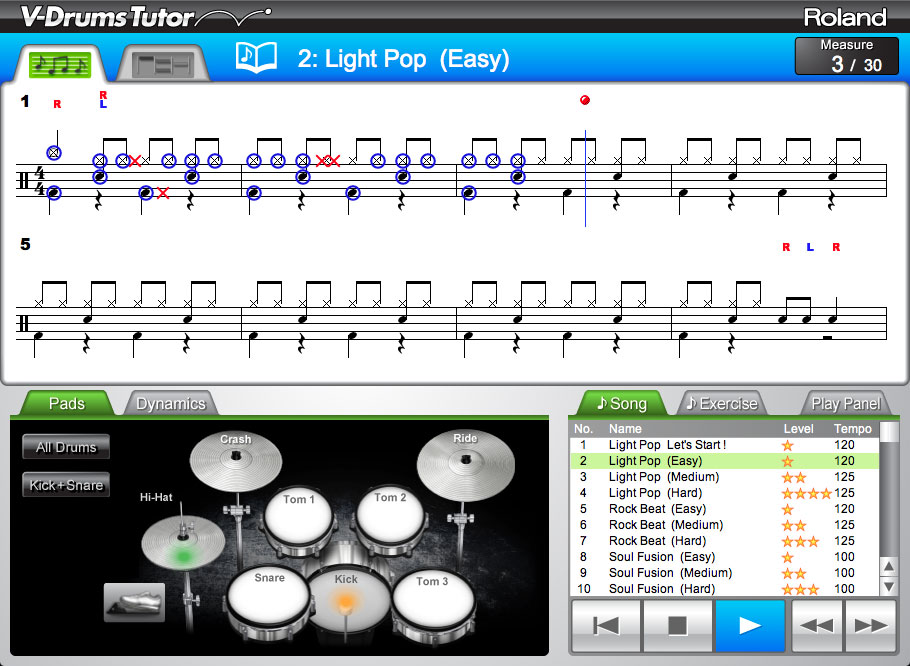
\includegraphics[scale=0.25]{dt-1_ss_main_notation_gal}
\end{figure}
\subsection{Beat Detection Background}

Detecting musical time is a skill which is not only fundamental to musicians [6] but also something that seemingly comes naturally to humans. The majority are able to analyse and reproduce the metre\footnote{Metre is the repeating pattern that provides the pulse of beat of a piece of music [12]}, tempo and rhythmic aspects of a piece of music [7]. Longuet-Higgins [6] was one of the first to produce an algorithm to replicate this human ability. He constructed a binary tree with each node representing a note or rest [8]. He then developed his theory into a system that was able to measure the variations in the downbeats of a piece of music and adjust the perceived tempo according to whether the note was later or earlier than expected [6]. Since Longuet-Higgins' first work there have been a number of different approaches to beat detection. M. Goto and Y. Muraoka developed a system which learned the frequencies of the bass drum and snare drum, in order to detect events triggered by these instruments during a piece of music [9]. In 2001, Simon Dixon presented Beatroot, an interactive beat tracking and visualisation system which is able to estimate the tempo and times of musical beats in performed music [10]. In the same year Tzanetakis \textit{et al} [11] described an algorithm based on the Discrete Wavelet Transform (DWT) which is capable of detecting the beat attributes of music. 


% Due to the rapidly expanding research being carried out on beat detection, the 1st annual Music Information Retrieval Evaluation eXchange (MIREX) was held in 2005. MIREX includes a contest with the goal of comparing state-of-the-art algorithms for music information retrieval [7]. The topics to be evaluated were proposed by the participants. In the first year, three of the nine topics concerned beat detection (Audio Drum Detection, Audio Onset Detection and Audio Tempo Extraction). 
% There are a number of pieces of software available for real time tempo detection is limited to only a few live bpm detectors available in the App Store\footnote{Apple's application store - itunes.apple.com/uk/appstore‎} and Google Play\footnote{Google's application store for Android devices - play.google.com/store}. An example It is therefore a focus of this project to investigate if the beat detection system Beatroot and Tzanetakis \textit{et al's} [12] method are accurate enough to be implemented in a live tempo drum beat analyser.

\subsubsection{Beatroot}
Beatroot is an audio beat detection system presented by Simon Dixon in 2001 and is described as a ``beat tracking system which finds the times of musical beats and tracks changes in tempo throughout a performance'' [13]. Beatroot works by first processing digital audio data to produce a list of onset (see Figure 2) or event times. The time intervals between these events are then analysed to generate tempo hypotheses concerning the rate and location of beats. Using the tempo hypotheses, searches are carried out to test the different hypotheses about the rate and timing of beats. The results of these searches are ranked and the beat times found in the highest ranked search are returned [10]. 

% \subsubsection{Onset Detection}
% Onset detection is a process used by most of beat detection methods currently available. The onset of a note is the instant which marks start of the variation in the frequency of a signal, a visualisation of this can be seen in figure 2. Once detected it can then be used to measure the onset times of sonic events\footnote{A sonic event is a singular feature of a piece music which can be made up of one source or many[24], e.g. the hitting of a drum} within a pieceof music [9].

\begin{figure}[h]
	\centering
	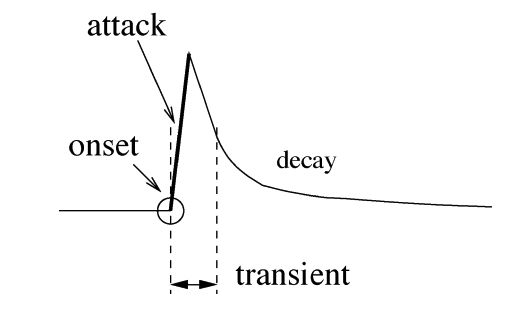
\includegraphics[scale=0.40]{Onset}
	\caption{The onset of a note is the instant which marks start of the variation in the frequency of a signal [11]}
\end{figure}

\subsubsection{Short-Time Fourier Transform}
To detect the onsets of a piece of digital audio Beatroot uses an onset detection function based on the Short-Time Fourier Transform (STFT). The STFT is a form of Fourier transform (FT) which was developed by Joseph Fourier in 1822 [16], which can be used to find out how much of each frequency exists in a signal. A drawback of the FT is that it is unable to provide any details of when a frequency component occurs in time for non-stationary signals\footnote{Non-stationary signals are signals whose frequency contents changes over time [17].}. A solution to this was to split a non-stationary signal up into a number of smaller segments using a window function, which effectively created a series of stationary\footnote{The frequency contents of a stationary signal does not change over time} signals which the FT could then be applied to. However, this did not fully solve the problem as the size of window function affects the quality of frequency resolution and time resolution:
\begin{itemize}
\item Narrow Window Function $\longrightarrow$  Good Time Resolution, Bad Frequency Resolution
\item Wide Window Function $\longrightarrow$  Bad Time Resolution, Good Frequency Resolution [17]
\end{itemize}

\subsubsection{Discrete Wavelet Transform}
The first literature regarding the wavelet was provided by the mathematician Albert Haar in 1909 [18]. The wavelet transform is a technique for analysing signals which was developed as an alternative to the STFT [11]. Like the STFT, the DWT is able to provide time and frequency information, however, unlike the STFT the DWT is able to do this without the need for a window function. 

\subsubsection{Tzanetakis \textit{et al} Beat Detection Method}
In 2001, Tzanetakis \textit{et al} described how the Discrete Wavelet Transform (DWT) could be used to extract information from non-speech audio [11]. Their beat detection algorithm was based on detecting the most prominent signals which are repeated over a period of time within the analysed audio and was is split into the following steps: 

\begin{enumerate}
\item Signal decomposed into a number of octave frequency bands using the DWT
\item The subsequent time domain information is extracted for each frequency band
\item The data from each band are then summed together and a function to find repeating patterns is applied
\end{enumerate}

As there is no current open source Java implementation of this algorithm. I will attempt to implement a version of this myself, which will be the DWT based beat detection component of this project.

\maketitle{}
\section{Aims and Objectives}
For my project I propose to build a real time drum beat tempo analyser. This will use the Beatroot system described previously and an implementation of the Tzanetakis \textit{et al}'s' beat detection algorithm [11]. This will form the basis of an investigation into whether these are suitable to be used in a live drumming tempo training tool. I will elaborate on the key features of this work in the following sections.


\subsection{Core Project Features}
\begin{itemize}
\item Live audio capturing and processing
\item Implement the beat detection algorithm described by Tzanetakis \textit{et al} [11] 
\item Build a system to record detailed comparative information regarding the efficiency and accuracy of Beatroot and Tzanetakis \textit{et al}'s algorithm in order to ascertain if they are accurate enough to be used in a training tool for drummers
\item Design a User Interface (GUI) to provide real time feedback on the current tempo played and beats detected
\item An extensive sample set of drum beats will need to be created to ensure the system is tested sufficiently
\end{itemize}

\subsection{Non-Core Project Features}
\begin{itemize}
\item Investigate if it is possible for the system to learn the frequencies of the different drums being played
\item Extend GUI to provide the user with real time notification on when a certain drum is played
\end{itemize}

\maketitle{} 
\section{Development Plan for the Solution}
A key part of my project involves the designing my own implementation of the beat detection algorithm described by Tzanetakis \textit{et al} [11]. This will then be incorporated in a beat detection system along with the Beatroot system in order to provide real time tempo analysis of an audio signal. 

\subsection{Proposed Architecture}

\begin{figure}[h]
	\centering
	\includegraphics[scale=0.60]{ProposedArch}
	\caption{Proposed architecture where the drum kit represents live audio flowing into the system.}
\end{figure}


\subsection{Live Audio Processing}
The live audio will be processed using the Javax Sound package. The audio will be captured using a stereo microphone and processed to match CD quality with the Javax Sound AudioFormat class. The Beatroot system was not originally intended to be used as a real time system [19] so currently only works with prerecorded audio. It will therefore be will need to be modified in order for it to work with live audio. 

% \begin{itemize}
% \item Encoding - This will be set to ``PCM.signed'', representing audio encoded to the native linear pulse code modulation, where quantization levels are linearly uniform [15].
% \item Sample Rate - 44,100, set to match CD quality for the number of analog samples which will be analysed per second. 
% \item Sample Size in Bits - 24, based on a sound card with a 24 bit sample depth.
% \item Channels - 2, audio will be captured using a stereo microphone.
% \item Frame Size - 6, where the frame size is the number of bytes in a sample multiplied by the number of channels [17].
% \item Frame Rate - 44,100, same as sample rate.
% \item Big Endian (boolean) - false, as the project will be developed on an Intel core which uses a little-endian architecture\footnote{Endianess refers to the order of bytes which make up a digital word. Big endianess stores the most significant byte at a certain memory address and the remaining bytes being stored in the following higher memory addresses. The little-endian formate reverses the order storing the least significant at the lowest and most significant at the highest memory address [16].}.
% \end{itemize}

\subsection{Implementation of Tzanetakis \textit{et al} Beat Detection Algorithm}
The beat detection algorithm described by Tzanetakis \textit{et al} [11] is based on detecting the most prominent periodicities of a signal and is made up of the following stages:\footnote{A full description of the theory regarding Tzanetakis \textit{et al} beat detection algorithm will be provided in the Project Report.}

\begin{itemize}
\item DWT - First the signal is processed by the DWT into a number of frequency bands 
\item Low Pass Filtering - a low pass filter is then applied to the signal in order to allow the lower frequencies of the signal to be analysed
\item Full Wave Rectification - each frequency band is then converted to one constant polarity (positive or negative)[wiki]. A visual representation can be seen in Figure 4
\item Downsampling - the sampling rate of the signal is decreased by an integer factor [20]
\item Normalisation - each band is then normalised using mean removal
\item AutoCorrelation - an autocorrelation function is then applied to the frequency bands, the first five peaks of this function are detected and their periodicities are calculated in beats per minute
\end{itemize}

\begin{figure}[h]
	\centering
	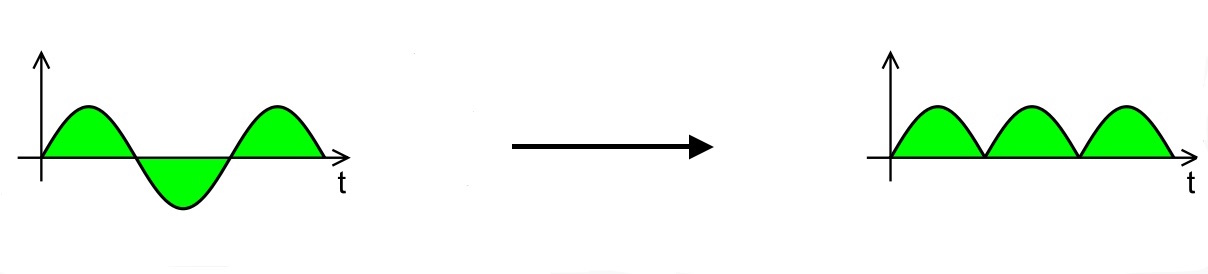
\includegraphics[scale=0.25]{FWR2}
	\caption{Visual representation of Full Wave Rectification (diagram adapting from https://en.wikipedia.org/wiki/Rectifier)}
\end{figure}

If the implementation of this algorithm takes longer than described in the schedule in   section 5. The Matlab implementation created by Eng Eder de Souza [21] will be adapted for use to be used in this system. 

\subsubsection{JWave}
The implementation of Tzanetakis \textit{et al} [11] beat detection algorithm will require the use of a library which provides DWT functionality. This will be provided by JWave. JWave is a Java library created by Christian Scheiblich which provides a number of different transform packages [22], including a wavelet package. For the purpose of this project the Daubechies wavelets classes within JWave will be used. The Daubechies wavelets are a form of discrete wavelet transform which were developed by Ingrid Daubechies in the late 1980's and are frequently used in applications [14]. 

\subsection{Comparative Analysis of Beat Detection Algorithms}
A key part of this project is to ascertain whether the two beat detection methods described in section 1 are accurate enough to create a training tool similar to the MIDI based software seen in figure 1. To achieve this the two systems will be run in parallel using real time audio and return details on the calculated tempo in beats per minute (bpm), the number of beats detected and the time it took to calculate the results. 
% The tempo will be the beats per minute (bpm) recorded at the end of each processed frame, all of the bpm's within the sample set will be exact and in order to match the current midi software packages accuracy any returned bpm's should be exact as well. However, very small deviations in tempo can be very hard to detect to the human ear so some margin of error will be applied. To account for the fact that at the slower bpm's any beat out of place will be a lot easier to hear than at a higher bpm, the margin for error will be weighted by using the following equation;

% \[ m = (bpm - 60) * 0.0001\]
% \begin{flushleft}
% where \(m\) represents the weighted value for the margin for error to be applied.
% \end{flushleft}
The data collected during this process will be recorded and stored in an appropriate format to allow it to be queried and analysed. Due to the relatively small amount of data which will be collected, it is not deemed necessary to create a database to store this. Instead the data will be stored in a JSON file. JSON was chosen over XML as it has a much simpler grammar and is able to map directly onto the data structures used in modern programming languages [23].

\subsection{Build Extensive Drum Sample Set}
The success of this project will rely heavily on the amount of live audio data that the system processes. A large set of drum beat samples will be required. The drum beats will be created using the Apple software package, Garageband. The sample set will contain beats from a variety of styles as well as samples with fluctuating tempos. The main aspects of the sample set are as follows:

\begin{itemize}
\item The tempo range will be 60 - 160 beats per minute. Some samples will be be created with varying tempos in order to model human playing more closely.
\item The time signatures will be mainly in common time (4/4) to reflect normal playing styles, however some drum beats will use swing notes\footnote{A swing note is style where notes with equal time are played with an unequal durations, usually as alternating long and short durations [wiki]} which will be created by feel\footnote{By adapting the strength a drum or cymbal is being played at it is possible to infer a different style of music using feel, e.g. swing time can be created this way.}.
\item Accenting\footnote{Accents are an emphasis placed on a specific note}, ghost notes\footnote{Ghost notes are a note which is played at a very low volume} and missed beats\footnote{Missed beats will be used to represent the drummer missing a drum or cymbal} will be added in line with a real playing style.
\item The sample set will contain a wide range of drum beats, including; beats using one drum, those only with a back beat, beats incorporating single rests within a bar or for the whole duration of a bar and beats with large solos and loud cymbal hits\footnote{When a cymbal is played at high amplitudes (loudness) the vibrations it create become chaotic and its clearly identifiable signals disappear and it effectively becomes noise [24]. It will therefore be interesting to see if this noise affects the accuracy of the algorithms in any way.}.
\end{itemize} 

The main musical styles will be rock and pop, blues and jazz. Approximately ten unique drum beats will be created for each style, which will then be sampled at a range of bpms. There will also be a final set of simple single and multiple drum beats included. The aim will be to generate a total set of approximately seven hundred and fifty samples.

\subsection{User Interface}
The user interface will be developed using the JavaFX framework, enabling the system will to be cross-platform compatible. Its features will be kept simple initially, where it will only be required to provide a real time output of the current two tempo calculations and accumulative count of beats detected.

\subsection{Non-Core Project Features}
The non-core project features will be included only if the project is developed ahead of the schedule described in section 5. 

\subsubsection{Frequency Learning}
This non-core feature will investigate if it is possible to create a similar system to the one developed by Goto and Muraoka, which learnt the frequencies of the snare and kick drum in order to detect events triggered when these instruments were played [6]. The goal will be to enable the system to learn the frequencies of all of the separate parts of a drum kit (snare drum, bass drum, tom-tom, hi-hat and cymbals) being played and use this event to extend the GUI.

\subsubsection{Extended User Interface}
Developing this additional feature will only be possible if the previous non-core feature (3.7.1) is successfully developed. If so, the user interface will be extended to look similar to the drum kit visual seen in Figure 1, where a colour indicator will be displayed to represent which instrument was last played. The development of this final feature depends heavily on the accuracy and efficiency of the tempo analysis algorithms used.

\subsection{Project Methodology}
This project will be developed using the Test Driven Development (TDD) framework. TDD is a development process that combines the test-first development and refactoring. Test-first development involves writing a test before just enough production code is written to fulfill that test [25]. Refactoring is the process of making small changes to code in order to improve its design, making it easier to understand and modify [26]. I intend to use TDD due to the relatively short development time of this project. TDD will enable small steps to be taken during the process which is considered to be a more productive approach to writing software [25].

\subsection{Development Languages and Testing}
The project will be developed in a combination of Java and Scala. Java is required as both the Beatroot and JWave libraries are in this language, however any functional aspects of the project will be developed in Scala, as it offers a superior functional tool set when compared to those offered in Java 8. As previously discussed JSON will be used to store the collected data.

I will use the Intellij IDE to develop this system. Git will be used for version control, testing will be completed using JUnit for Java, and Scala Test for any functionality developed in Scala. In order to ensure that the parsed JSON is well formed it will be tested using the JSON validator found at - http://jsonlint.com/.

\section{Challenges, Probability, Impact and Mitigation}
The challenges associated with this project and their mitigation can be found in Table 1.
\begin{table}[h]
\caption{Key Project Challenges and Mitigation} 
\centering
\begin{tabular}{|p{6cm}|p{6cm}|c|c|}
 \hline
\textbf{Challenge} & \textbf{Mitigation} & \textbf{Probability} & \textbf{Impact}\\ [0.5ex]
\hline 
Own implementation of Tzanetakis \textit{et al} [11] beat detection algorithm takes longer than expected & Adapt the Eng Eder de Souza Matlab implementation instead & Medium & High\\
\hline
Beatroot does not configure to work with real time audio & Find and use an alternative & Low & High\\ 
\hline
The two beat detection systems do not integrate well in a concurrent system & Create a two separate systems & Low & High\\
\hline
Not enough time to develop the GUI & Develop simple command line based user interface & Low & Low\\
\hline
\end{tabular}
\end{table}

\clearpage
\maketitle{} 
\section {Project Schedule}
The start date for the project is Monday 13th June 2016 and the end date is Monday 19th September 2016, the non-core project features will only be completed if the project is ahead of schedule.
\begin{table}[h]
\caption{Project Timeline} 
\centering
\begin{tabular}{|p{4cm}|p{8cm}|}
 \hline
\textbf{Dates} & \textbf{Task}\\ [0.5ex]
\hline 
w/c 13th June 2016 & Develop live audio capturing system\\
\hline 
w/c 20th June 2016 & Set up Beatroot library in development environment\\
\hline 
w/c 27th June 2016 & Implement DWT beat detection algorithm in Scala/Java\\
\hline 
w/c 4th July 2016 & Test systems with single live audio source\\
\hline 
w/c 11th July 2016 & Develop system to store data generated during tempo analysis\\
\hline 
w/c 18th July 2016 & Research and build appropriate framework to process captured audio in parallel e.g. akka actors\\
\hline 
w/c 1st August 2016 & Create sample set of drum beats\\
\hline 
w/c 8th August 2016 & Test system using full sample set\\
\hline 
w/c 15th August 2016 & Develop UI\\
\hline 
w/c 22nd August 2016 & Analyse logged data\\
\hline 
w/c 29th August 2026 & Write up report\\
\hline 
w/c 5th September 2016 & Present findings to project supervisor\\
\hline 
w/c 12th September 2016 & Finalise report\\
\hline 
w/c 19th September 2016 & Submit report\\
\hline
\end{tabular}
\end{table}
\clearpage
\maketitle{} 
\section{Summary}
I propose to build a real-time drum beat tempo analysis system using the Short-Time Fourier Transform based Beatroot library and an implementation of the Tzanetakis \textit{et al} [11] beat detection algorithm. An extensive set of drum samples will then processed through the system to represent live audio and the results recorded. These results be analysed to determine if the two beat detection methods are suitable to be implemented in a real time training tool for drummers.


\maketitle{} 
\section{References}
\begin{enumerate}
\item https://en.wikipedia.org/wiki/Downbeat
\item https://en.wikipedia.org/wiki/Bar\_(music)
\item http://www.instructables.com/id/What-is-MIDI/ %22
\item https://en.wikipedia.org/wiki/Time\_signature
\item http://www.roland.co.uk/blog/exploring-roland-dt-1-v-drums-tutor-software/ %1
\item Allen and Dannenberg (1990), Tracking Musical Beats in Real Time, International Computer Music Conference, International Computer Music Association, pp. 140-143 %2
\item P. Desain and H. Honing (1989), The Quantization of Musical Time: A Connectionist Approach, Computer Music Journal, Vol. 13 No. 3 (Autumn), pp. 56-66 %3
\item H. C Longuet-Higgins (1976), Perception of melodies, Nature Vol. 263, pp. 646-653 %4
\item M. Goto and Y. Muraoka (1994), A beat tracking system for acoustic signals of music, in Proceedings of the Second ACM International Conference on Multimedia, pp. 365-372 %5
\item S. Dixon (2001), Automatic Extraction of Tempo and Beat from Expressive Performances, Journal of New Music Research, 30 (1), pp. 39-58. %6
\item G. Tzanetakis, G. Essl and P. Cook (2001), Audio Analysis using the Discrete Wavelet Transform, Proc. WSES International Conference on Acoustics and Music: Theory and Applications (AMTA) %12
\item https://en.wikipedia.org/wiki/Metre\_(music)
\item S. Dixon (2003), On the Analysis of Musical Expression in Audio Signals, Storage and Retrieval for Media Databases, SPIE-IS\&T Electronic Imaging, SPIE Vol. 5021, pp. 122-132 %13
\item Andreas de Vries (2006), Wavelets, FH Sudwestfalen University of Applied Sciences %27
\item Juan Pablo Bello, Laurent Daudet, Samer Abdallah, Chris Duxbury, Mike Davies, and
Mark B. Sandler (2005), IEEE TRANSACTIONS ON SPEECH AND AUDIO PROCESSING, VOL. 13, NO. 5, pp. 1035 - 1047
\item https://en.wikipedia.org/wiki/Fourier\_transform
\item http://users.rowan.edu/~polikar/WAVELETS/WTpart2.html %10 
\item Gao, Robert X, Yan, Ruqiang (2011), Wavelets, Theory and Applications for Manufacturing %26
\item Simon Dixon (2007), Evaluation of the Audio Beat Tracking System BeatRoot, Preprint for Journal of New Music Research, 36 %29
\item http://uk.mathworks.com/help/signal/ref/downsample.html
\item https://github.com/ederwander/Beat-Track %20
\item https://github.com/cscheiblich/JWave
\item http://www.json.org/xml.html %21
\item http://www.soundonsound.com/sos/may02/articles/synthsecrets0502.asp
\item http://www.agiledata.org/essays/tdd.html
\item http://www.agiledata.org/essays/databaseRefactoring.html
% \item http://www.music-ir.org/mirex/wiki/2005:Main\_Page %7
% \item https://en.wikipedia.org/wiki/Onset\_(audio) %8
% \item http://www.music-ir.org/mirex/wiki/2016:Audio\_Onset\_Detection %9

% \item http://users.rowan.edu/~polikar/WAVELETS/WTpart4.html %11


% \item https://en.wikipedia.org/wiki/Discrete\_wavelet\_transform %14
% \item https://en.wikipedia.org/wiki/Pulse-code\_modulation %15
% \item https://en.wikipedia.org/wiki/Endianness %16
% \item http://www.jsresources.org/faq\_audio.html %17
% \item https://en.wikipedia.org/wiki/Test-driven\_development %18
% \item A. Robertson, A. Stark and M. E. P. Davies (2013), Percussive Beat tracking using real-time median filtering, 6th International Workshop on Machine Learning and Music %19
% \item http://disp.ee.ntu.edu.tw/tutorial/WaveletTutorial.pdf %23
% \item http://www.ieor.berkeley.edu/~ieor170/sp15/files/Intro-to\_Sonic\_Events\_Campion.pdf %24



% \item Simon Dixon (2001), An Interactive Beat Tracking and Visualisation System %28


% \item Graham Percival, Member, IEEE, and George Tzanetakis (2014) %32
% \item http://dictionary.onmusic.org/appendix/topics/meters %33
\end{enumerate}
\end{document}
